% Chapter Template

\chapter{Implementation} % Main chapter title

\label{Chapter4} % Change X to a consecutive number; for referencing this chapter elsewhere, use \ref{ChapterX}
In this section we explain in detail, what hardware we used in our implementation and with which technology the UWB communication and ranging was done. Finally we briefly explain the core of our work, the mathematical theory of the particle filter.

%----------------------------------------------------------------------------------------
%	SECTION 1
%----------------------------------------------------------------------------------------

\section{Hardware}
We decided to use Raspberry Pis for all mobile devices such as the TAG and the ANs. As the Raspberry Pis were not equipped with UWB technology, we extended them with a SEQUITUR Pi board from UNISET company running InGPS Lite firmware. In the following two subsections we present you these two hardware components.

%-----------------------------------
%	SUBSECTION 1
%-----------------------------------
\subsection{Raspberry Pi}
A Raspberry Pi is a single-board computer not much bigger than a credit card. Raspberry Pis are mainly designed for educational purposes as an alternative to expensive notebooks or desk computers. Hence the focus lies also on easy-to-use and plug-and-play experiences. Raspberry Pis are useful for versatile types of projects, as they provide common state of the art hardware - like HDMI, USB and wireless LAN - direct on boad and as they are extendable with selected components.

We used Raspberry Pi Model B \cite{Raspberry}, these were the most relevant specifications for our work:
\begin{itemize}
\item Quad Core 1.2GHz Broadcom BCM2837 64bit CPU
\item1GB RAM
\item 100 Base Ethernet
\item 40-pin extended general purpose input output (GPIO)
\item Micro SD port for loading your operating system and storing data
\end{itemize}

%-----------------------------------
%	SUBSECTION 1
%-----------------------------------
\subsection{SEQUITUR Pi board with InGPS Lite}
On the 40-pin extended GPIO, we connected the SEQUITUR Pi board from UNISET Company. UNISET is a company located in Italy that focuses on research, development and manufacturing of innovative sensors in two major application areas \cite{Uniset}:
\begin{itemize}
\item Access control security systems, enhancing the reliability of intrusion detection
\item Indoor and outdoor tracking. Sequitur is a precise real time locating system (RTLS) for tracking any object in 2D or 3D with centimeter accuracy.
\end{itemize}
This hardware seemed perfect for our ambitions, as it provides a state-of-the-art UWB communication and ranging. Moreover the SEQUITUR Pi board of the TAG has IMU sensors like 3D-accelerometer and 3D-magnetometer on board. With the boards, UNISET delivers a firmware running on Raspberry Pis operating system (OS) to establish a connection via user datagram protocol (UDP). This firmware allows to communicate with the sensors in order to retrieve IMU sensor data, but also to get direct access to the range between two nodes. It is explained in detail throughout the next section. 

%----------------------------------------------------------------------------------------
%	SECTION 2
%----------------------------------------------------------------------------------------

\section{UWB Communication and Ranging}
The theoretical design on our system is shown in \ref{fig:system_design}, it works as follows:
At least three ANs, equipped with UWB technology, are placed in an indoor environment of one floor. Our algorithm runs on a seperate server, where a zoneplan and floorplan of the floor are available. A single TAG is located somewhere on the floor, it is as well equipped with UWB technology, moreover it measures acceleration and magnetic energy with the onboard IMU. The TAG continously collects data from the IMU and contemporary waits for a request from the server. The server periodically requests data via UWB from the TAG. As soon as a request is noticed at the TAG, it performs a range estimation to every AN and sends this data together with the continously collected IMU data to the server.
For every estimation period, the server has all the data needed to feed the particle filter.

%-----------------------------------
%	SUBSECTION 1
%-----------------------------------
\subsection{Transmission}
Here goes the text.


\begin{figure}[th]
\centering
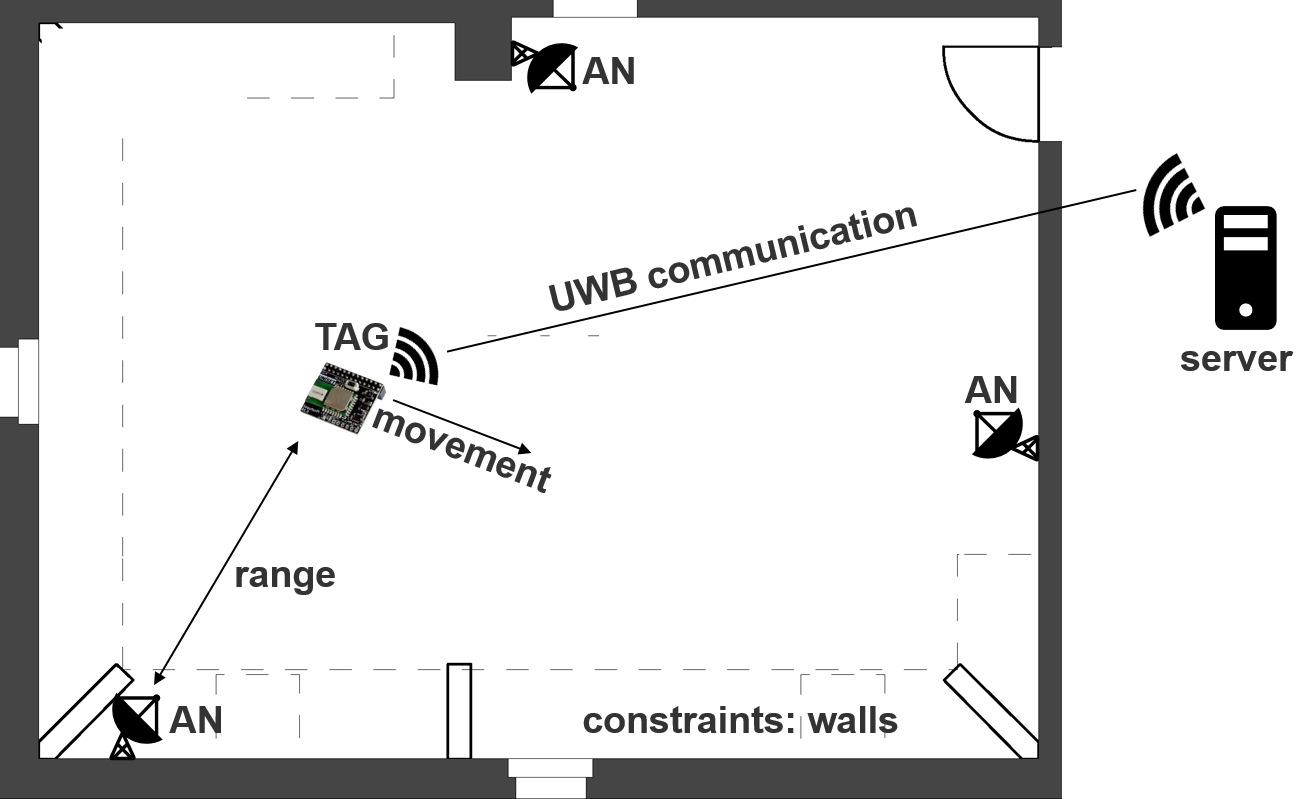
\includegraphics[width=1.0\textwidth]{Figures/system_design}
\decoRule
\caption[System Design]{Overview of the theoretical system design.}
\label{fig:system_design}
\end{figure}

%-----------------------------------
%	SUBSECTION 2
%-----------------------------------
\subsection{Ranging with TWR}
Here goes the text.

%----------------------------------------------------------------------------------------
%	SECTION 3
%----------------------------------------------------------------------------------------

\section{Particle Filter}
All computations are done on the seperate server, as we would like to minimize the required computational power and energy consumption of the devices. As already mentioned, the server receives IMU data and range estimations from the nodes. This data, as well as the floorplan constraints and the zone indication, flow into the particle filter. These operations are done on the server:
\begin{itemize}
\item Spread the particles and validate new positions with floormap constraints
\item Evaluate UWB ranges, IMU measures and zone indication to assign likelihood
\item Calculate weight function and systematically resample (and reposition) particles with low weights
\item Sum up weighted positions
\end{itemize}

%-----------------------------------
%	SUBSECTION 1
%-----------------------------------
\subsection{Inputs}
Here goes the text.

In the first part, every particle is moved from its current to a new position. To validate the new position, we check if the direct trajectory between the old and the new location intersects with an impediment. If so, a new position is generated, as the last was not reachable.
The second item covers the likelihood of the new position. For every AN, the measured distance is compared to the distance from the new position to the AN. The less these two distances differ, the higher is the assigned liklihood. This is also in effect for the IMU motion, as the difference between the old and the new positon is compared to the measured IMU motion to evaluate the likelihood. \textbf{@Mischa:ADD PART OF ZONE INDICATION} % Add zone indication part!
In the weighting step, every particle gets weighted by the liklihoods of the previous computations. The weights of all particles are normalized for further processing.
The last part is simply a weighted sum of the particles locations.

%-----------------------------------
%	SUBSECTION 2
%-----------------------------------
\subsection{Likelihood and weighting}
Here goes the text.


%-----------------------------------
%	SUBSECTION 3
%-----------------------------------
\subsection{Ranging with TWR}
Here goes the text.